\documentclass[12pt]{report}
\usepackage{ECE_Dissertation_Style}
\usepackage{amsmath,amssymb,latexsym,float,epsfig,subfigure,overpic}
%these margins allow you to use the default "shrink oversize pages" option when printing
\usepackage[lmargin=1.40 in, rmargin=0.86 in,tmargin=1.0 in,bmargin=1.0 in]{geometry}
\usepackage{indentfirst}
\usepackage{afterpage}
\usepackage{sectsty}
\usepackage{hyperref}
\usepackage{caption}
\usepackage{etoolbox}
%%% bookmarks - color them black
\hypersetup{
	colorlinks=true,
	citecolor=black,
	filecolor=black,
	linkcolor=black,
	urlcolor=black
}
%Set graphics path
\graphicspath{{./pictures/pdf/},{./pictures/ps/},{./pictures/png/},{./pictures/jpg/}}
\captionsetup{format=hang}
%Fill pages with text and floats
\renewcommand\textfraction{.1}
\renewcommand\topfraction{.9}
\renewcommand\bottomfraction{.7}
\renewcommand\floatpagefraction{.7}
%Remove white space above chapter headings
\makeatletter
\patchcmd{\@makechapterhead}{\vspace*{50\p@}}{}{}{}% Removes space above \chapter head
\patchcmd{\@makeschapterhead}{\vspace*{50\p@}}{}{}{}% Removes space above \chapter* head
\makeatother


\begin{document}

%Set limits on font sizes for headings
\chapternumberfont{\fontsize{16}{20}\selectfont}
\chaptertitlefont{\centering\fontsize{16}{20}\selectfont}
\sectionfont{\fontsize{14}{16}\selectfont}
\subsectionfont{\fontsize{12}{14}\selectfont}

%%
%%
\title{Applications of Unmanned Vehicles with Wireless Sensor Networks and Surveying} %% If you want to specify a linebreak
                               %% in the thesis title, you MUST use
                               %% \protect\\ instead of \\, as \\ is a
                               %% fragile command that \MakeUpperCase
                               %% will break!
\author{Anne Smith}
\department{Department of Electrical and Computer Engineering}

%% Can have up to four readers in addition to the advisor.
%% All have the form
%%
%%  \reader{Name}[Department][Institution]
%%
%% The second and third arguments are optional, but if you wish to
%% supply the third, you must supply the second. Department defaults
%% to the department defined above and Institution defaults to a blank.

\advisor{Aaron T. Becker, Assistant Professor}[Department of Electrical Engineerign]
\firstreader{Matthew Franchek , Professor}[Department of Mechanical Engineerign]
\secondreader{Miao Pan, Assistant Professor}[Department of Electrical Engineerign]
%\setcounter{secnumdepth}{2}
\degree{Master of Science}
\major{Electrical Engineering} 

\copyrighttrue
\copyrightyear{2018}
\submitdate{August 2018} % Must be the month and year of graduation,
                         % not thesis approval! As of 2010, this means
                         % this text must be May, August, or December
                         % followed by the year.

%defaults to thesis option
\dissertationfalse

%%%%%%%%%%%%%%%%%%%%%%%%%%%%%%%%%%%%%%%%%%%%%%%%%%%%%%%%%%%%%%%%%%%%%%%%%%%%%%%
% COVER PAGES:  Flyleaf, copyright page, title page, signature page
%
\makecoverpages

%%%%%%%%%%%%%%%%%%%%%%%%%%%%%%%%%%%%%%%%%%%%%%%%%%%%%%%%%%%%%%%%%%%%%%%%%%%%%%%
% ACKNOWLEDGMENTS
%
% Put acknowledgments in a file called "ack.tex" and it'll be inputted here.
\begin{acknowledgements}

% acknowledgements for thesis

Thank you to Dr. Aaron Becker, for giving me the opportunity to work on these beautiful projects, with these fascinating people.
You are an excellent example of a professor who cares about his student and his teaching as much as his research.
I hope the lab continues to grow after I graduate.
I hope I graduate.

Thank you to the lab members who came and went during my time here, for putting up with me.
Thank you for allowing me to be a lab manager my way, even though it might not have been the most friendly way.
I hope you are able to utilize this lab we have built together for a long time.
%Thank you to the Master students from our lab who came before me, to show me that it is possible.
%Thank you to the our lab's undergraduate students, some of you have become Master students with me.
%Should jazz this up a bit

Thank you to my collaborators, who put up with me when, by my own choice, I worked alone on our collaboration.

Thank you to my parents, Tung Thanh Trinh and Binh Van Nguyen, and my sister, Duong Thuy Nguyen.
Mom, you sacrificed your professional and social life for our family.
I regret not being able to spend as much time with you when I was in school, I hope that will change soon.
Dad, the stories of your struggles showed me that it can work out if I keep going, and with a little bit of luck, or the ancestors' blessing, as you put it.
Thank you for giving us a better life, and the opportunity to do what I love.
I hope I can be proud of myself as you are of me.
I hope I give you guys less headache.
Duong, thank you for showing me that you don't have to be successful in school to be successful in life.
I wish you and Juan to be happy and fulfilled the rest of your life.
I am very grateful that you decide to share that happiness with me.

\end{acknowledgements}

%%%%%%%%%%%%%%%%%%%%%%%%%%%%%%%%%%%%%%%%%%%%%%%%%%%%%%%%%%%%%%%%%%%%%%%%%%%%%%%
% ABSTRACT
%
% Put acknowledgments in a file called "abs.tex" and it'll be inputted here.
\abstitlep
\abstractsection

% abstract for thesis

This is the abstract.  It has a limit of 150 words for a masters thesis and 350 words for a PhD dissertation.



%%%%%%%%%%%%%%%%%%%%%%%%%%%%%%%%%%%%%%%%%%%%%%%%%%%%%%%%%%%%%%%%%%%%%%%%%%%%%%%
% TABLE OF CONTENTS
%
% print table of contents, figures and tables here.
\makecontentspages
%%

\prefacesection

%%%%%%%%%%%%%%%%%%%%%%%%%%%%%%%%%%%%%%%%%%%%%%%%%%%%%%%%%%%%%%%%%%%%%%%%%%%%%%%
% INSERT REAL CONTENT HERE
%
% Thesis Introduction

\chapter[Introduction]{Introduction}
\label{chap-intro}

\section[Autonomous Unmanned Vehicles]{Autonomous Unmanned Vehicles}

Since the industrial revolution, autonomous machines have become a significant contributor to increased human productivity.
From the steam engine and assembly line conveyor belt, autonomous machines take over repetitive, labor-intensive tasks and leave human with jobs requiring more attention to details but less physical energy.
Every year, the list of tasks automated by machines grow bigger.
Vehicles were one of the first few machines predicted to be automated, yet Autonomous Unmanned Vehicles (AUV) just recently became commercially available, although in smaller scales.

With the advent of commercially available small AUV, we can automate tasks such as surveying, sensor network distribution, and inspection, which previously require intensive human labor.
Surveying with visual, sonar and laser sensor with Unmanned Aerial Vehicles (UAV) have become commercially available.
UAV photography is growing into a booming business, with turn key solution packages.
Enabling photo and movie studios to get aerial footage and pictures without the need for expensive helicopter rentals.
UAV surveying with traditional or modified surveying equipment reduces the cost of surveying sites for constructions or archeological digs.


\section[Seismic AUV] {Deploying seismic microphones with AUV}

\begin{figure}
\centering
\begin{overpic}[width=\columnwidth]{ral2016/intro.pdf}\end{overpic}
\caption{\label{fig:Hetero_overall}
	The heterogeneous sensor system presented in chapter \ref{chap:SeismicDarts}: wireless SeismicDarts and a SeismicSpider, both designed for UAV deployment. 
}
\end{figure}

Seismic microphones are used in seismic surveying to find subsurface deposits of natural resources.
Seismic surveying can also be used to identify where earthquakes can happen.
Traditionally, seismic microphones are connected $\SI{2}{\metre}$ or $\SI{3}{\metre}$ apart on a long cable.
The cable is composed of 20 to 30 microphones and connected to one computer responsible for recording the reflected sound wave.
Several cables can be laid out to cover the entire survey area, so the length of cable required is proportional to survey area.
Transporting the cables means increased weight, and they can be difficult to maneuver and deploy on rough terrain.
Surveyors will need to expand a lot of manual labor to distribute these sensors

Recently, nodal sensors with their own recording unit can be used, eliminated the need for cabling.
However, these nodal sensors are still planted and recovered by hand, requiring surveyors to traverse rough terrain multiple times.

Our first use of AUV is to make nodal seismic microphone deployable from an Unmanned Aerial Vehicle (UAV).
Our system can be seen in Fig.~\ref{fig:Hetero_overall}.
The SeismicDart is a dart shaped, wireless capable sensor that can be dropped from a UAV to plant into the ground firmly.
The SeismicSpider is a mobile six-legged robot rover with three seismic microphones for legs.
The Spider can be deployed in a clearing where UAVs can access, then walk into a more covered area were it's hard for UAV to fly over and drop SeismicDarts.
The system can be utilized to quickly deploy sensor asset for geoscience research~\cite{werner2006deploying} such as
earthquake~\cite{dominici2012micro},
and volcano \cite{nagatani2013volcanic} monitoring,
defense operations~\cite{wu2007efficient},
and wildlife monitoring~\cite{dyo2010evolution,mainwaring2002wireless}. 

\section[Mosquito AUV]{Destructive surveying of mosquito with UAV}

\begin{figure}
	\centering
	\begin{overpic}[width=1\columnwidth]{icra2018/DroneAndNet_v2.pdf}\end{overpic}
	\caption{\label{fig:DroneAndNet}
		A hexacopter UAV carrying a $\SI{48}{\centi\metre} \times \SI{61}{\centi\metre}$ rectangular bug-zapping screen.
		An onboard microcontroller monitors the voltage across the screen and records the time, GPS location, humidity, and altitude for each mosquito strike.
		At right are three frames recorded by the onboard camera showing mosquito hits, during the day (top) and at twilight.
		See attachment for videos of flight experiments~\cite{Bhatnagar2018}.
	\vspace{-2em}
	}
\end{figure}

Mosquito-borne diseases kill millions of humans each year~\cite{murray2012global}. 
Because of this threat, governments worldwide track mosquito populations.
Following individual mosquitoes is difficult because of their small size, wide-ranging flight, and preference for low-light.
Tracking studies of individual mosquitos have chosen to use small ($\SI{1.2}{\metre} \times \SI{2.4}{\metre}$) indoor regions~\cite{parker2015infrared}, or mating swarms backlit against a solid background~\cite{butail20113d}.

The dominant tools for tracking mosquito populations are stationary traps that are checked at weekly intervals (\textit{e.g.,} Encephalitis Vector Surveillance traps and/or gravid traps~\cite{williams2007comparison}). 
Recent research has focused on making these traps smaller, cheaper, and capable of providing real-time data~\cite{chen2014flying,linn2016building}; however, they still rely on attracting mosquitoes to the trap. 
We present an alternate solution using an electrified bug-zapping screen mounted on an unmanned aerial vehicle (UAV) as shown in Fig.~\ref{fig:DroneAndNet} to seek out the mosquitoes in their habitat.
As the UAV follows a path, it sweeps out a volume of air, temporarily removing all the mosquitoes in this volume.
By monitoring the voltage across this screen, we can track individual mosquito contacts.
UAVs have strict energy budgets, so optimized flight patterns are of crucial importance.
As a consequence, putting the UAV to good use requires methods for computing trajectories that minimize energy consumption along the way, but maximize the total volume of mosquitoes at visited locations.

\section[Drifting sensors]{Surveying underwater with drifting sensors}

\begin{figure}[h]
	\begin{center}
	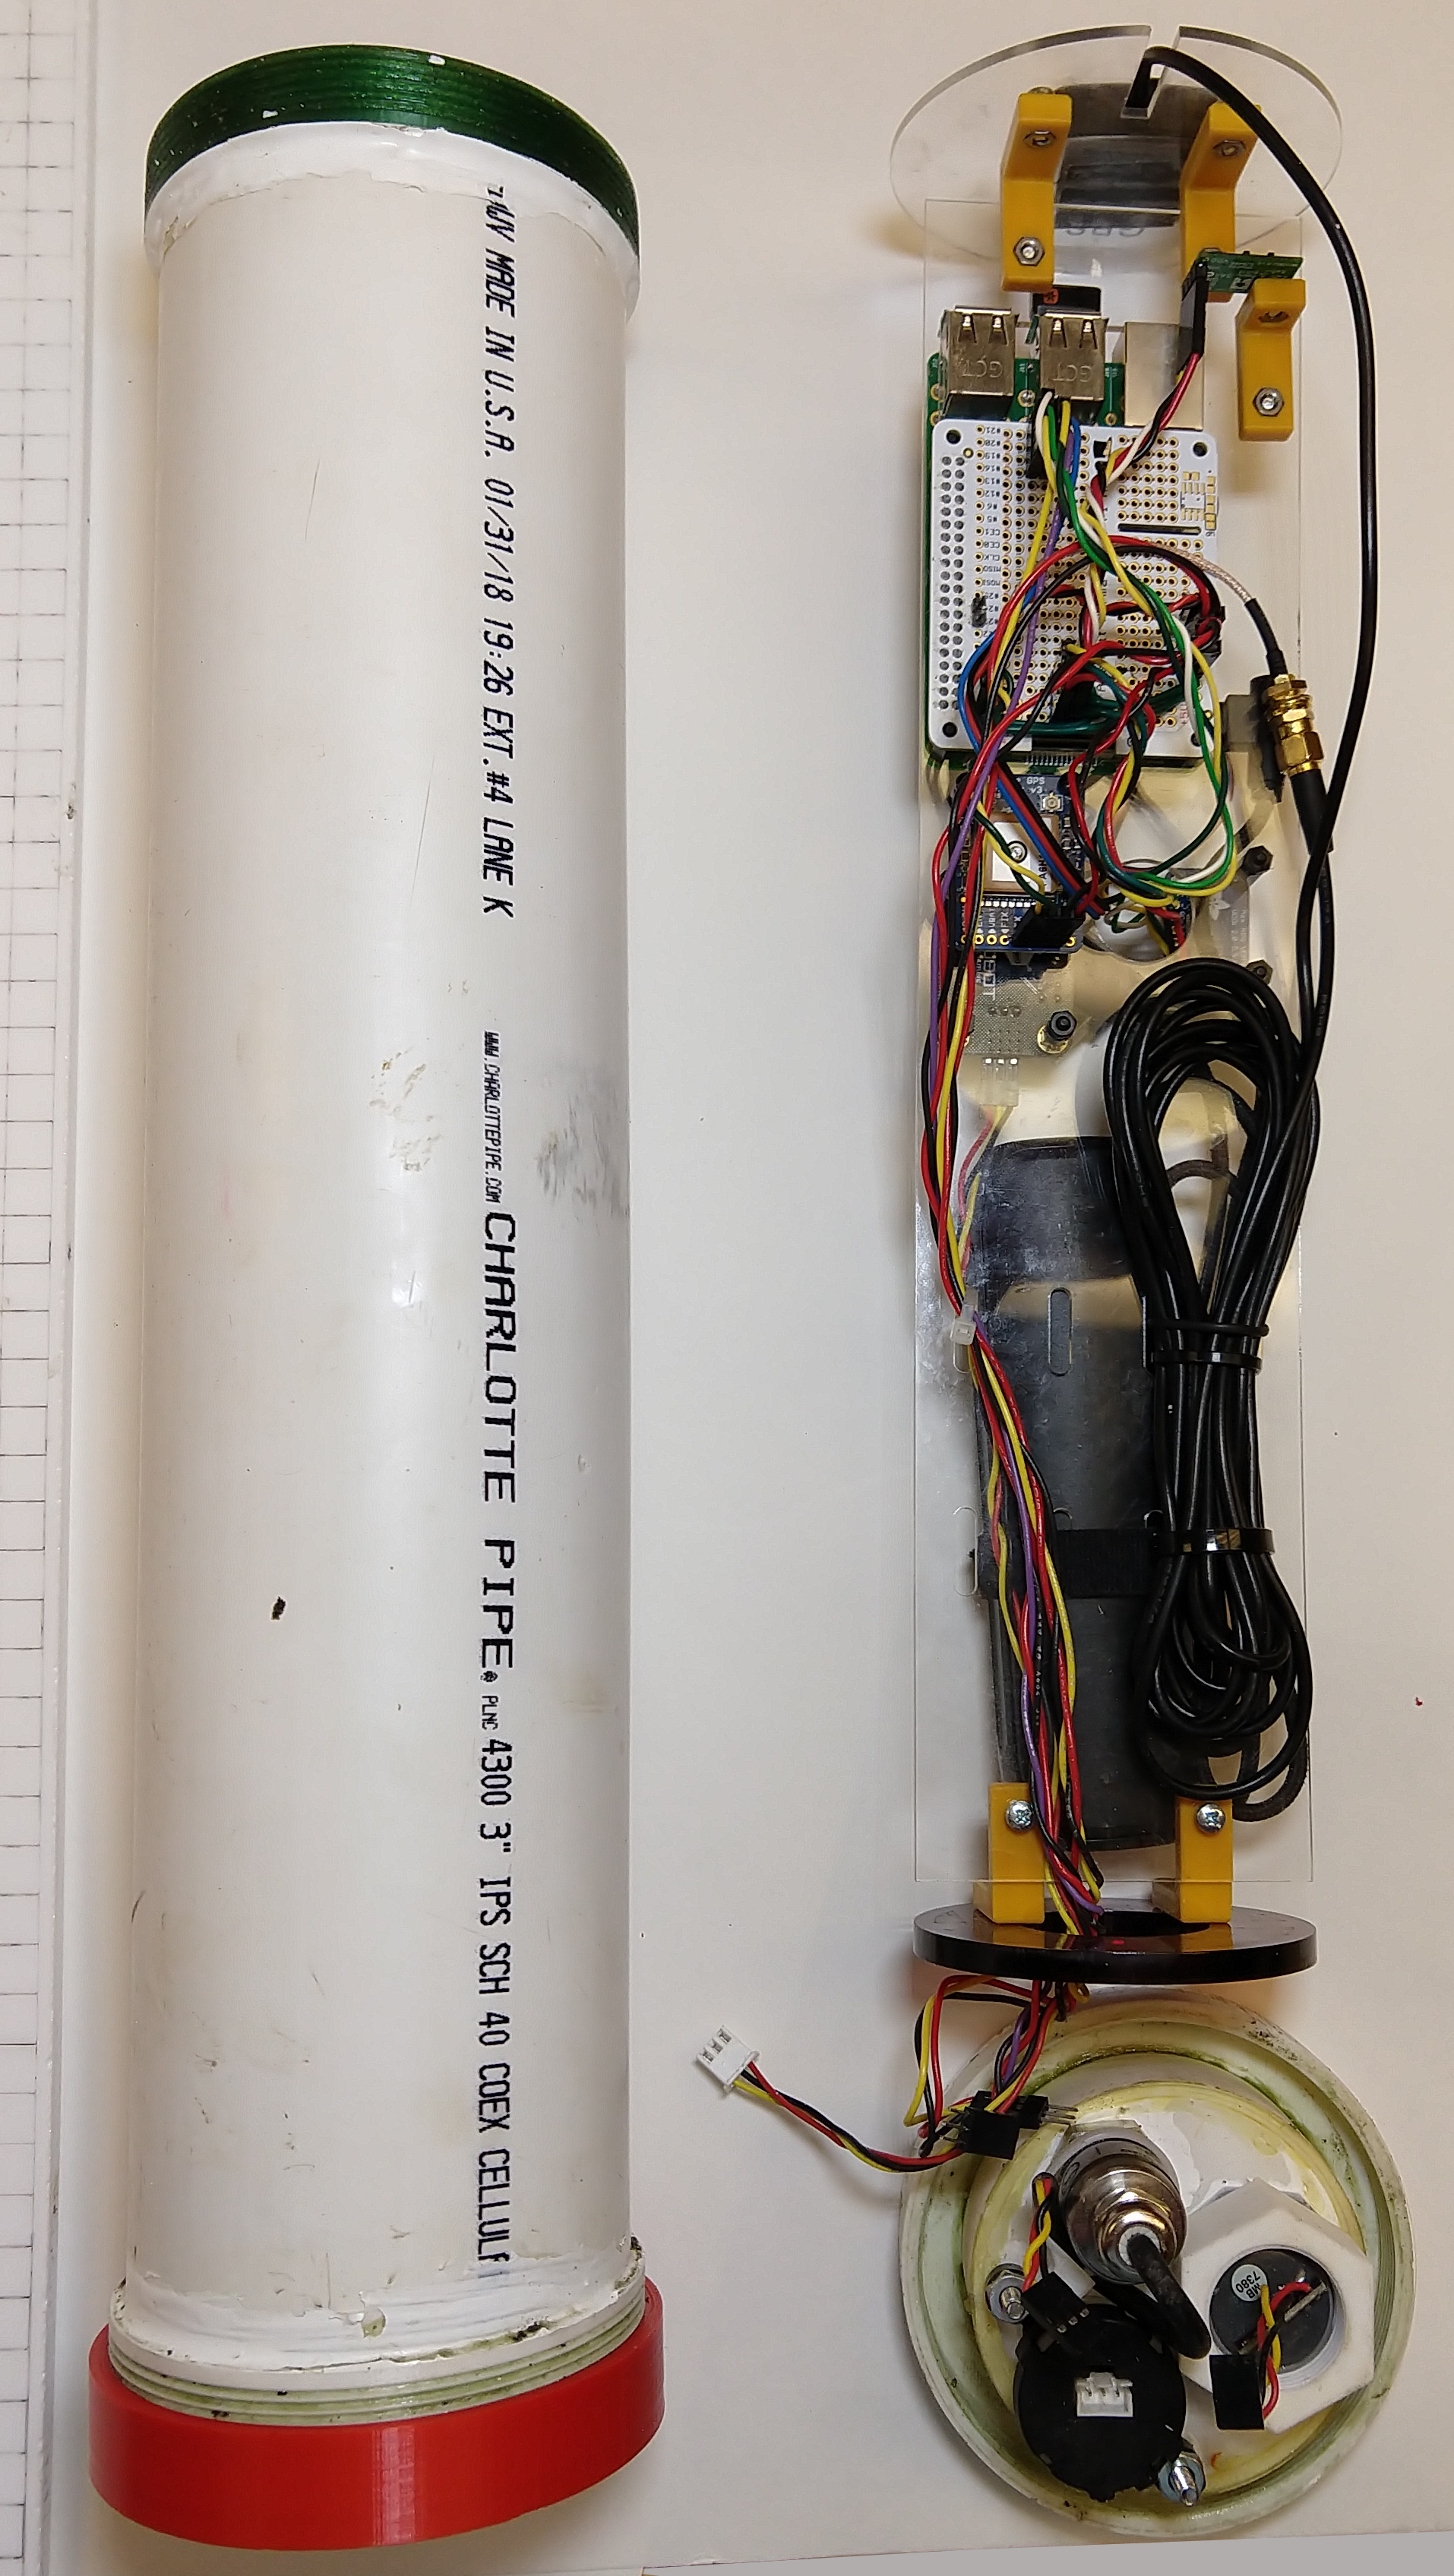
\includegraphics[height=12cm]{driftnode/driftnode.jpg}
	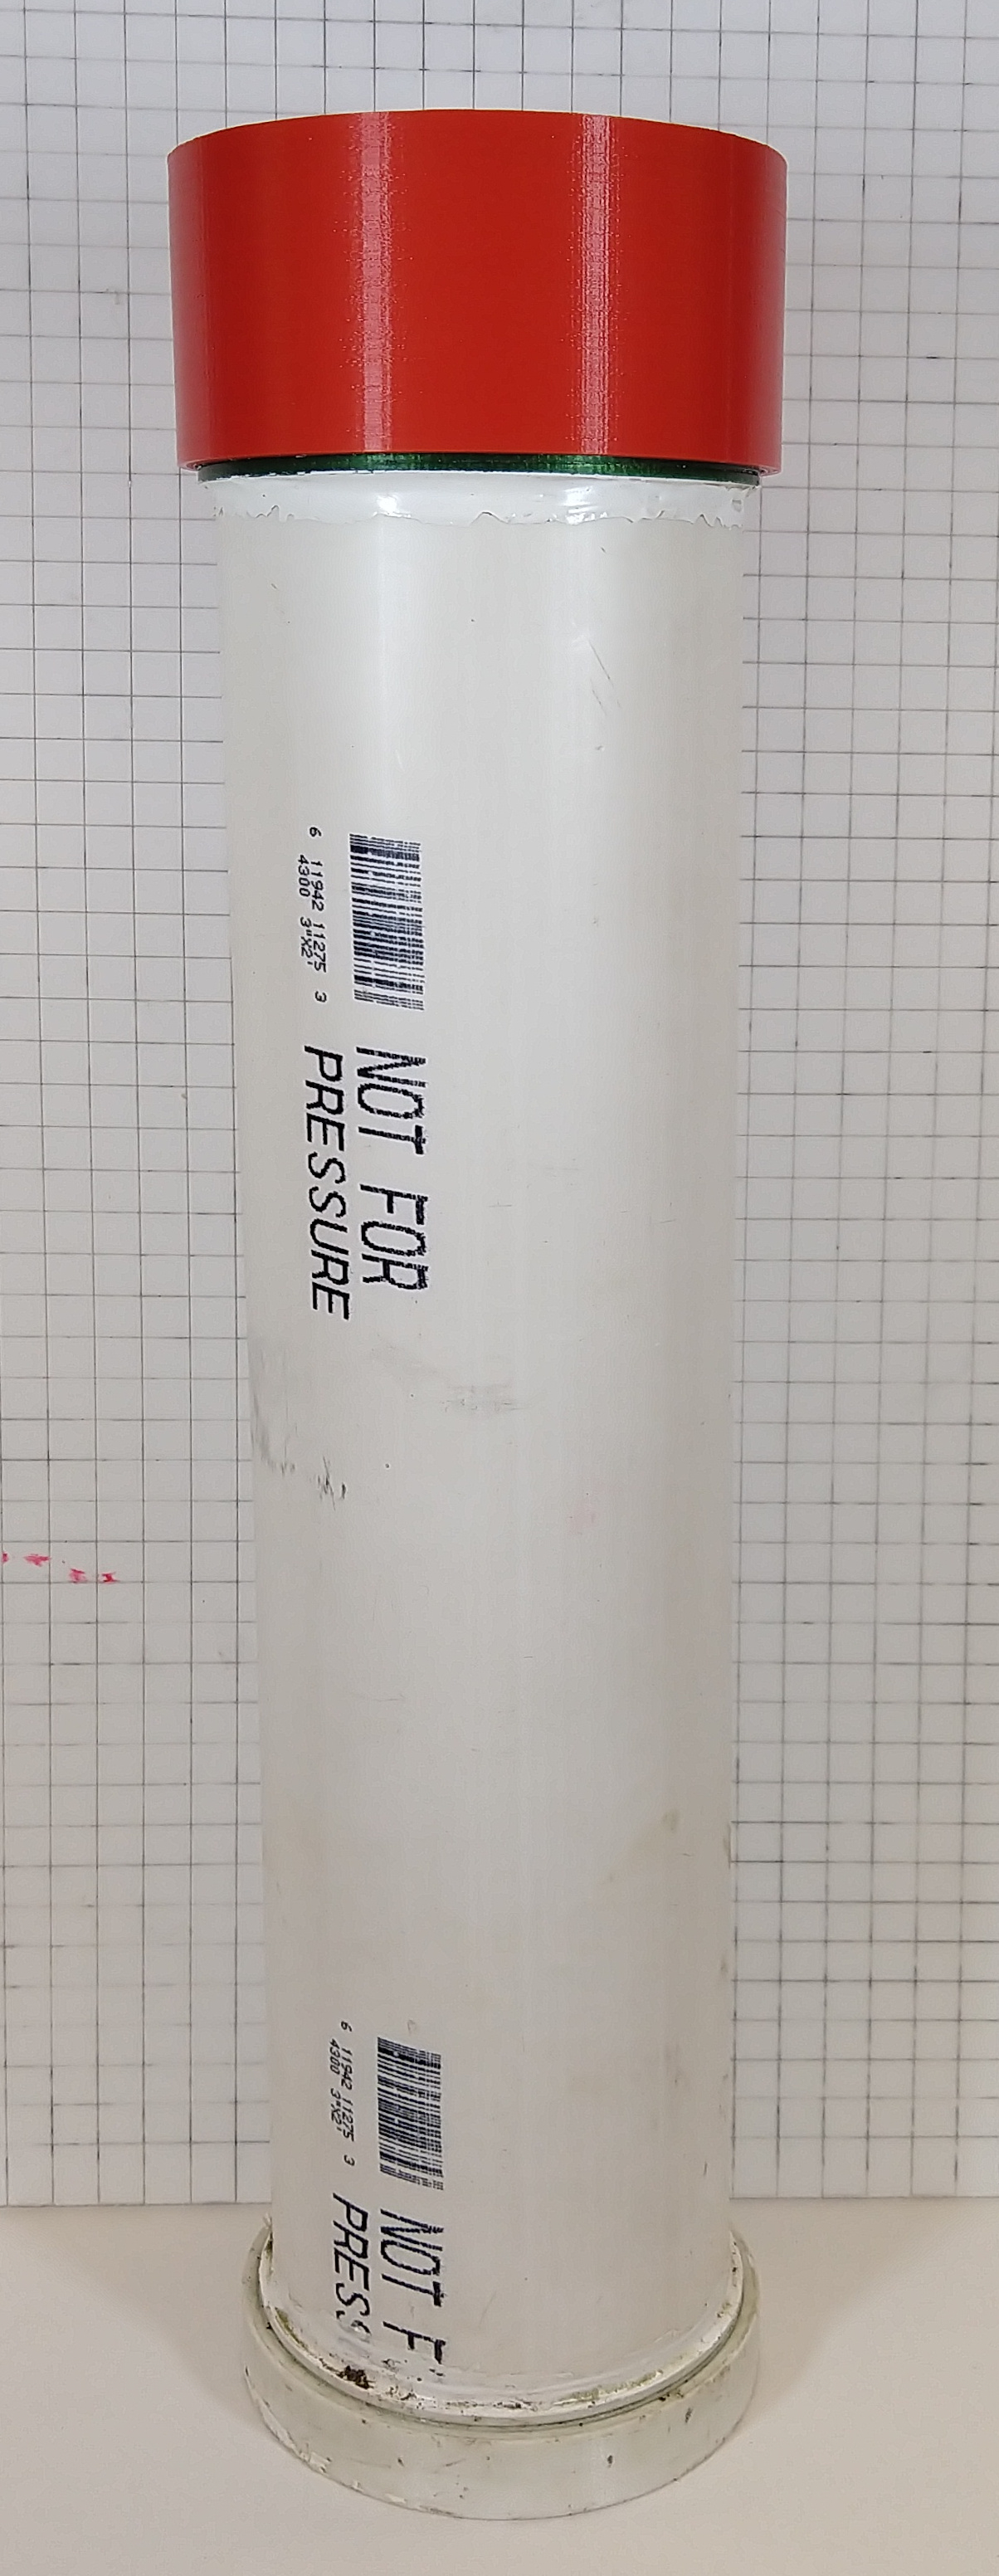
\includegraphics[height=12cm]{driftnode/driftnodeassembled.jpg}
	\caption[Driftnode]{
		(Left) driftnode before assembly, the electronics are attached to a center acrylic plate.
		(Right) an assembled driftnode.
	} \label{fig:driftnodeoverview}
	\end{center}
	\vspace{-1em}
\end{figure}

Humans knows less about the ocean than they do about space.
Because EM waves attenuate quickly in water, it is challenging to deploy wireless sensor network in water for permanent surveying post.
A boat and crew need to be dispatched to survey a water surface.
The crew can then manually deploy sensor at each location within the area for scientific research.
The team will need to be dispatched periodically to monitor an area for border security or fishing enforcement.
One crew cannot watch several areas simultaneously, so the man-hour required grow proportionally with area monitored.
This requires the need for several crews, or risk security incidence when an area is not monitored.

A wireless sensor network, composed of drifting sensors, deployed temporarily or permanently, can monitor an area for much longer with less labor needed.
A UAV can be used to periodically visit these sensors, collecting their sensor logs and charging them.
We present a drifting sensor platform, initially created by the University of South Carolina \cite{drifterUSC}, as seen in Fig.~\ref{fig:driftnodeoverview}.
The drifting sensor is composed of a suite of underwater sensor: An underwater depth sensor, a pressure sensor, a turbidity sensor, 9-axis IMU and GPS location sensor.
Our drifting sensor can broadcast its own wireless access point, which enables an AUV to collect data from the sensor at close range.

\chapter[Results]{Results}\label{chap-results}

Here's the discussion of the results.  You can add as many chapters as you like.
% Thesis 

\chapter[Conclusion]{Conclusion}
\label{chap-conc}

In this thesis, three applications for autonomous unmanned vehicles were presented.
Unmanned aerial vehicles (UAV) can be used to deploy, retrieve geophones for seismic surveying and deploy unmanned rover attached with geophones.
We presented software to plan for a wireless sensor network deployment using UAV and unmanned rover.
A UAV was used to drag an electrified net through an area to destructively survey mosquito populations.
We used our collaborator's algorithm to reduce the energy expenditure while maximizing area covered.
An updated design for drifting wireless sensor node was presented.
The drift node can be used to survey coastlines and national maritime boundaries for marine border security, wildlife science missions.

In future work, the applications above could be merged together for a more complete package.
A wireless sensor network can then be deployed, monitored and retrieved by AUVs.
Before the WSN deployment, the area can be surveyed by a UAV with minimal energy expenditure.
Wireless sensor nodes can communicate with each other to relay position, cache data or relay data back to the base station.
Like in \cite{sudarshanwsn}, UAVs can monitor data and charge wireless sensor nodes, extending their longevity.
For destructive mosquito surveying methods, the UAVs can incorporate live data to plan its route reactively.

%We developed a method to deploy geophones for seismic surveying with AUVs, reducing manual labors and injury risks.
%The geophones are combined with a data recording unit, can record its own position and the soundwave during the seismic survey.
%This eliminate long analog data transmisison cables, which reduce a large part of equipment weight during surveying.
%We can drop geophones from our UAVs when we put the geophones a SeismicDart shell, which eliminates the need for a separate UAV per sensor.
%For terrains that UAVs cannot fly to or the SeismicDart cannot approach, we developed a SeismicSpider, with geophones for legs.
%The SeismicSpider can travel to its desired position, with geohphones contacting the ground, record the soundwave during the survey.
%The software we developed to schedule a seismic survey can be used for many other wireless sensor network applications that use UAVs and autonomous rovers.



\bibliographystyle{IEEEtran}
\addcontentsline{toc}{chapter}{References}
\bibliography{IEEEabrv,thesisrefs}

%any appendices go here

\afterpage{\blankpage}
\end{document}
